\documentclass{article}
% packages
\usepackage{amsmath,amssymb}
\usepackage{graphicx}
\usepackage{hyperref}

% directory of figures
%\graphicspath{ {figs} }

% latin bold lower
\newcommand{\ba}{\mathbf{a}}
\newcommand{\bc}{\mathbf{c}}
\newcommand{\be}{\mathbf{e}}
\newcommand{\bh}{\mathbf{h}}
\newcommand{\bp}{\mathbf{p}}
\newcommand{\bt}{\mathbf{t}}
\newcommand{\bs}{\mathbf{s}}
\newcommand{\bu}{\mathbf{u}}
\newcommand{\bv}{\mathbf{v}}
\newcommand{\bw}{\mathbf{w}}
\newcommand{\bx}{\mathbf{x}}
\newcommand{\by}{\mathbf{y}}
\newcommand{\bz}{\mathbf{z}}
\newcommand{\bm}{\mathbf{m}}

% latin bold upper
\newcommand{\bA}{\mathbf{A}}
\newcommand{\bB}{\mathbf{B}}
\newcommand{\bC}{\mathbf{C}}
\newcommand{\bI}{\mathbf{I}}
\newcommand{\bJ}{\mathbf{J}}
\newcommand{\bL}{\mathbf{L}}
\newcommand{\bM}{\mathbf{M}}
\newcommand{\bP}{\mathbf{P}}
\newcommand{\bQ}{\mathbf{Q}}
\newcommand{\bR}{\mathbf{R}}
\newcommand{\bT}{\mathbf{T}}
\newcommand{\bU}{\mathbf{U}}
\newcommand{\bV}{\mathbf{V}}
\newcommand{\bW}{\mathbf{W}}
\newcommand{\bX}{\mathbf{X}}
\newcommand{\bY}{\mathbf{Y}}
\newcommand{\bZ}{\mathbf{Z}}

% latin cal upper
\newcommand{\cF}{\mathcal{F}}
\newcommand{\cG}{\mathcal{G}}
\newcommand{\cI}{\mathcal{I}}
\newcommand{\cL}{\mathcal{L}}
\newcommand{\cM}{\mathcal{M}}
\newcommand{\cN}{\mathcal{N}}
\newcommand{\cS}{\mathcal{S}}
\newcommand{\cT}{\mathcal{T}}
\newcommand{\cW}{\mathcal{W}}
\newcommand{\cX}{\mathcal{X}}
\newcommand{\cZ}{\mathcal{Z}}

% latin bb upper
\newcommand{\bbE}{\mathbb{E}}
\newcommand{\bbI}{\mathbb{I}}
\newcommand{\bbP}{\mathbb{P}}
\newcommand{\bbR}{\mathbb{R}}
\newcommand{\bbX}{\mathbb{X}}
\newcommand{\bbY}{\mathbb{Y}}
\newcommand{\bbW}{\mathbb{W}}

% greek bold lower
\newcommand{\bepsilon}{\boldsymbol{\epsilon}}
\newcommand{\btheta}{\boldsymbol{\theta}}
\newcommand{\blambda}{\boldsymbol{\lambda}}
\newcommand{\bpi}{\boldsymbol{\pi}}
\newcommand{\bmu}{\boldsymbol{\mu}}
\newcommand{\bsigma}{\boldsymbol{\sigma}}
\newcommand{\bphi}{\boldsymbol{\phi}}

% greek bold upper
\newcommand{\bSigma}{\boldsymbol{\Sigma}}

\DeclareMathOperator*{\argmin}{arg\,min}
\DeclareMathOperator*{\argmax}{arg\,max}

% transpose
\newcommand{\T}{^{\text{\tiny\sffamily\upshape\mdseries T}}}


% if you need to pass options to natbib, use, e.g.:
\PassOptionsToPackage{numbers, sort, compress}{natbib}
% before loading neurips_2025


% ready for submission
%\usepackage{neurips_2025}


% to compile a preprint version, e.g., for submission to arXiv, add add the [preprint] option:
\usepackage[preprint]{neurips_2025}


% to compile a camera-ready version, add the [final] option, e.g.:
%\usepackage[final]{neurips_2024}


% to avoid loading the natbib package, add option nonatbib:
%\usepackage[nonatbib]{neurips_2024}


\usepackage[utf8]{inputenc} % allow utf-8 input
\usepackage[T1]{fontenc}    % use 8-bit T1 fonts
\usepackage{hyperref}       % hyperlinks
\usepackage{url}            % simple URL typesetting
\usepackage{booktabs}       % professional-quality tables
\usepackage{amsfonts}       % blackboard math symbols
\usepackage{nicefrac}       % compact symbols for 1/2, etc.
\usepackage{microtype}      % microtypography
\usepackage{xcolor}         % colors

%%%

\usepackage{subcaption}
\usepackage{graphicx}
\usepackage{multirow}
\usepackage{amsmath,amssymb,amsfonts}
\usepackage{amsthm}
\usepackage{mathrsfs}
\usepackage{xcolor}
\usepackage{textcomp}
\usepackage{manyfoot}
\usepackage{booktabs}
\usepackage{algorithm}
\usepackage{algorithmicx}
\usepackage{algpseudocode}
\usepackage{listings}

\newtheorem{theorem}{Theorem} % continuous numbers
%%\newtheorem{theorem}{Theorem}[section] % sectionwise numbers
%% optional argument [theorem] produces theorem numbering sequence instead of independent numbers for Proposition
\newtheorem{proposition}[theorem]{Proposition}% 
\newtheorem{lemma}{Lemma}% 
%%\newtheorem{proposition}{Proposition} % to get separate numbers for theorem and proposition etc.

\newtheorem{example}{Example}
\newtheorem{remark}{Remark}

\newtheorem{definition}{Definition}
\newtheorem{assumption}{Assumption}

%%%

\title{Neural Networks Loss Landscape Convergence in Different Low-Dimensional Spaces}


% The \author macro works with any number of authors. There are two commands
% used to separate the names and addresses of multiple authors: \And and \AND.
%
% Using \And between authors leaves it to LaTeX to determine where to break the
% lines. Using \AND forces a line break at that point. So, if LaTeX puts 3 of 4
% authors names on the first line, and the last on the second line, try using
% \AND instead of \And before the third author name.


\author{
  Tem Nikitin\\
  Moscow Institute of Physics and Technology\\
  Moscow, Russia\\
  \texttt{nikitin.artem.a@phystech.su}\\
  \And
  Nikita Kiselev\\
  Moscow Institute of Physics and Technology\\
  Moscow, Russia\\
  \texttt{kiselev.ns@phystech.su}\\
  \And
  Andrey Grabovoy\\
  Moscow Institute of Physics and Technology\\
  Moscow, Russia\\
  \texttt{grabovoy.av@phystech.su}\\
  \And
  Vladislav Meshkov\\
  Moscow Institute of Physics and Technology\\
  Moscow, Russia\\
  \texttt{meshkov.ns@phystech.su}\\
}


\begin{document}

\maketitle

\begin{abstract}
  Understanding how the loss landscape of neural networks evolves as the training set size increases is crucial for
  optimizing performance. It is well known that larger datasets can alter the shape of this high-dimensional landscape.
  But the exact point at which additional data no longer brings substantial changes remains underexplored.

  In this paper, we examine neural network models and show that their loss landscapes begin to stabilize once the
  training set grows beyond a certain threshold, revealing a connection between dataset size and the geometry of the
  loss surface. To understand this phenomenon, we propose a method that projects the full parameter space onto a
  low-dimensional subspace derived from top eigenvectors of the Hessian. That provides a more interpretable view of how
  the loss surface in the vicinity of local minima behaves as more data become available. We use different sampling
  strategies, applying Monte-Carlo estimation to capture the structure of this reduced loss landscape more precisely.

  We validate our insights through experiments on image classification tasks, demonstrating that this low-dimensional
  analysis can reveal when the landscape effectively settles, and thus helps determine a minimum viable dataset size.
  Our findings shed light on the relationship between dataset scale and optimization geometry, and suggest
  practical strategies for balancing computational costs with the benefits of additional training data.
\end{abstract}

\textbf{Keywords:}
Neural networks, Loss landscape, Low-dimensional subspace, Hessian eigenvectors, Monte Carlo estimation, Dataset size threshold.

\section{Introduction}\label{sec:intro}

Neural networks have become irreplaceable in various aspects of life and have a lot of applications now
(e.g. image classification, language models, recommender systems, etc.). However, as datasets and models grow larger and
larger, we get higher accuracy and breakthrough results. However some problems connected with computation resources have
appeared. Sometimes models have so many parameters so we need time we cannot provide for their training. Some attempts to
explore and compare optimization methods have already been made \cite{soydaner2020comparison}. The core problem of all these
solutions hides in their locality, as the size of the neural network and training dataset remains unchanged. In this paper we
explore when adding more data no longer brings significant improvements in network performance and to explain
obtained results in terms of the curvature and shape of the neural network’s loss landscape.

Our research on the loss landscape of neural networks. Specifically, how it changes while adding new samples
to the training dataset. There remains a problem: processing of large datasets requires a lot of time.
We need to determine when increasing dataset size stops reshaping this loss landscape for general neural networks.
But the question of a minimum viable dataset size --- a threshold beyond which further data bring insignificant changes ---
remains underexplored. Moreover, connecting such a threshold to generalization capabilities \cite{wu2017towards} will
reduce computation requirements as we show that there is an upper bound of "active" dataset samples.

We suggest using the Hessian of the loss function to calculate its close approximation. However, the computation of all
Hessian requires a bunch of time, so we consider a projection of neural network parameters space to a certain subspace.
We place the following tasks to the front:
\begin{enumerate}
  \item Constructing a Hessian-based projection of the loss landscape which finds main curvature directions
        (top eigenvectors) in parameter space.
  \item Using different sampling methods, identifying at which dataset size the shape of the loss function stabilizes.
  \item We apply visualization methods to characterize the loss landscape next to the local minima.
  \item Providing applicable theoretical criteria to determine when adding more samples has minimal effect.
        We refer to The Matrix Cookbook \cite{petersen2012matrix} as a hint for matrix operations.
\end{enumerate}

The proposed solution is novel as it links Hessian estimation to the idea of a minimal dataset threshold. This enables
advantages such as more cost-effective dataset collection and a clearer understanding of how dataset size interacts with the
geometry of the loss function. And applying recent methods for low-rank Hessian estimation
can speed up and solve the problem of high computation cost of top eigenvalues for very large networks.

We validate our analysis results on well-known image classification tasks like MNIST \cite{deng2012mnist} and Fashion-MNIST
\cite{xiao2017fashion}. By connecting practical results to theoretical bounds, we offer a method for identifying
a computation-efficiency method that balances performance with accuracy gains.

\textbf{Contributions.} Our contributions can be summarized as follows:
\begin{itemize}
  \item We present a Hessian-based approach that uses a projection into a low-dimensional subspace of top eigenvectors to
        find the critical sufficient dataset size.
  \item We demonstrate the validity of our theoretical framework through empirical studies on MNIST and Fashion-MNIST,
        incrementally increasing dataset size until additional data makes an impact to the loss function curvature.
  \item We highlight the implications of our findings for practical data collection strategies, showing how the detection of
        a sufficient dataset size can reduce computation time.
\end{itemize}

\textbf{Outline.} The rest of the paper is organized as follows. Section 2 divides existing results into some
topics, highlighting their key contributions and findings. Section 3 considers general notation and
some preliminary calculations. In Section 4, we provide theoretical bounds on the hessian and losses
difference norms. Empirical study of the obtained results is given in Section 5. We summarize and
present the results in Sections 6 and 7. Additional experiments and proofs of theorems are included
in the Appendix A.

\section{Related Work}\label{sec:rw}

\textbf{Hessian-based analysis.}
The landscape of loss functions has been explored from various perspectives in the literature. Methods connected with Hessian
are central to understanding the convergence process and loss function landscape \cite{kiselev2024unraveling}. Recent works
observed that the Hessian of some models tends to have a low effective rank, with only a small quantity of eigenvalue
differences from zero. Empirical explorations from \cite{sagun2018empirical} show that the Hessian rank is often very low in
the vicinity of local minima, highlighting a significantly smaller “active subspace”.
Prior work investigating how large eigenvalues emerge during training \cite{ghorbani2019investigation}.

Some results have already been reached for fully connected and convolutional architectures \cite{meshkov2024convnets},
but they need generalization.


\textbf{Loss Landscape Geometry.}
Other recent researches aimed at how dataset size affects both performance and the geometry of loss function landscapes.
In the assumption of enough training samples, neural networks often reach smoother and flatter minima with better
generalization \cite{wu2017towards}. However, collecting large datasets is expensive, as well as the computation
requirements for them, raising questions about the most effective ratio between dataset and model sizes
\cite{hoffmann2022training}. As understanding the landscape of loss functions is key to the solution, prior work has looked
at visualizing loss surfaces \cite{li2018visualizing}.

\section{Preliminaries}\label{sec:prelim}

\subsection{General notation}

In this section, we introduce the general notation used in the rest of the paper and the basic assumptions.

We consider a $K$-label classification problem.
So, let's consider $p(y|\bx)$ a conditional probability, which maps unobserved variable $\bx \in \bX$ to the corresponding
output $y \in \by$. We consider $\by$ is a subspace (or same space) as $\mathbb{R}^K$. Let $f_{\bw}(\cdot)$
be a neural network with a list of parameters $\bw$. Let $\bOmega$ be a space of parameters ($\bw \in \bOmega$).

Let
$$\mathcal{D} = \left\{ (\bx_i, y_i) \, | \, i = 1, \dots, m \right\}$$
be a given dataset of size $m$ consists of i.i.d.
samples. Let $\ell(\cdot, \cdot)$ be a given loss function (e.g. cross-entrophy) where first argument refers to neural network's
result and the second argument refers to the true answer. To simplify, define:
$$\ell_i(\bw) := \ell(f_{\bw}(\bx_i), y_i).$$

\begin{definition}
  The empirical loss function for the first $k$ elements is:
  $$\cL_k(\bw) = \frac1M \sum\limits_1^k \ell_i(\bw), \,\, \cL(\bw) := \cL_m(\bw).$$
\end{definition}

Thus, the difference between losses for neighbouring samplem sizes is:
$$\cL_{k+1}(\bw) - \cL_{k}(\bw) = \frac{\ell_{k}(\bw) - \cL_{k-1}(\bw)}{k}.$$

\begin{definition}
  Let the Hessian of $\cL_k(\bw)$ be:
  $$\bH_k(\bw) = \nabla^2_{\bw}\cL_k(\bw) = \frac1k \sum\limits_1^k \nabla^2_{\bw} \ell_i(\bw).$$
\end{definition}

\begin{definition}
  To calculate the overall loss landscape changing, one has to integrate the absolute difference for the entire parameter space.
  We define $\mathbf{\Delta}$-\textbf{function} (delta-function) as:
  $$\Delta_{k} = \int \left( \cL_{k+1}(\bw) - \cL_{k}(\bw) \right)^2 p(\bw) dw,$$
  where $p(\bw)$ describes the priority of the particular parameter points so we can make $p(\bw)$ have higher values
  next to the local minima.
\end{definition}

We firther investigate this difference and aimed at exploration of how adding a new object to the dataset changes the value.
We interested in convergence of this value and properties of loss function when the training dataset size limits to $\infty$.

\begin{definition}
  Let $\Delta$ be a positive hyperparameter that indicates the stop-difference for $\Delta_k$. If
  $$k^* = \inf\limits_k\{\forall m \geq k: \, \Delta_m < \Delta\}$$
  we can say that $k^*$ samples in the dataset are enough to describe the distribution of data from the general population.
  We call $k^*$ as \textbf{sufficient}.
\end{definition}

\subsection{Assumptions}

\begin{assumption}
  Let $\bw^*$ be the local minimum of both $\cL_{k-1}(\bw)$ and $\cL_{k}(\bw)$.
  Thus, $$\nabla \cL_{k+1}(\bw^*) = \nabla \cL_{k}(\bw^*) = 0.$$
\end{assumption}

This assumption allows us to explore the behavior and the geometry of the loss function landscape at only one point.

Furthermore, using second-order Taylor's approximation for $\cL_{k}(\bw)$ at $\bw^*$ we get:
$$\cL_{k}(\bw) \approx \cL_{k}(\bw^*) + \frac12 (\bw - \bw^*)^{\T} \bH_k(\bw^*)(\bw - \bw^*)$$

\begin{assumption}
  We can assume that $\bw^*$ is a local minimizer, so that $\cL_{k+1}(\bw^*) = \cL_k(\bw^*)$.
\end{assumption}

\begin{assumption}
  We can assume parameters $\bw$ to be random, which will lead to quite natural condition: $p(\bw)$ can be even a prior
  distribution of $\bw$, so:
  $$\Delta_{k} = \mathbb{E}_{p(\bw)} \left( \cL_{k+1}(\bw) - \cL_{k}(\bw) \right)^2 = $$
  $$\mathbb{D}_{p(\bw)} \left( \cL_{k+1}(\bw) - \cL_{k}(\bw) \right) + \left( \mathbb{E}_{p(\bw)} \left(
      \cL_{k+1}(\bw) - \cL_{k}(\bw) \right) \right)^2$$
\end{assumption}

\section{Method: Projection onto Dominant Eigen-Directions and Loss Landscape Approximation}

Working with the full Hessian $\mathbf{H}_k(\bw)$ of a neural network is computationally expensive due to the high dimensionality
of the parameter space $\bOmega$. To overcome this issue, we reduce the complexity by projecting the parameters onto a lower-dimensional
subspace. This subspace is spanned by the $d$ dominant eigenvectors of the Hessian evaluated at the local minimum $\bw^*$, i.e.,
$\mathbf{H}_k(\bw^*)$.

The core idea behind the projection is that, in neural network models, the Hessian has a low effective rank according to
\cite{sagun2018empirical}: only a few eigenvalues are significantly larger than zero, while the majority are negligibly small.
As a result, the directions corresponding to these small eigenvalues contribute little to the variation of the loss
function. By keeping only the eigen-directions associated with the largest eigenvalues, we obtain a compact but informative
representation of the loss landscape that captures the most influential directions of curvature.

For further intuition, we present an experimental result on the plot \ref{fig:evgen} showing the dependence of the eigenvalues
on their index (ordered in descending order). The dominant eigenvalues were computed iteratively using a method described in
\cite{hessian-eigenthings}.

\begin{figure}[!htbp]
  \centering
  \subfloat{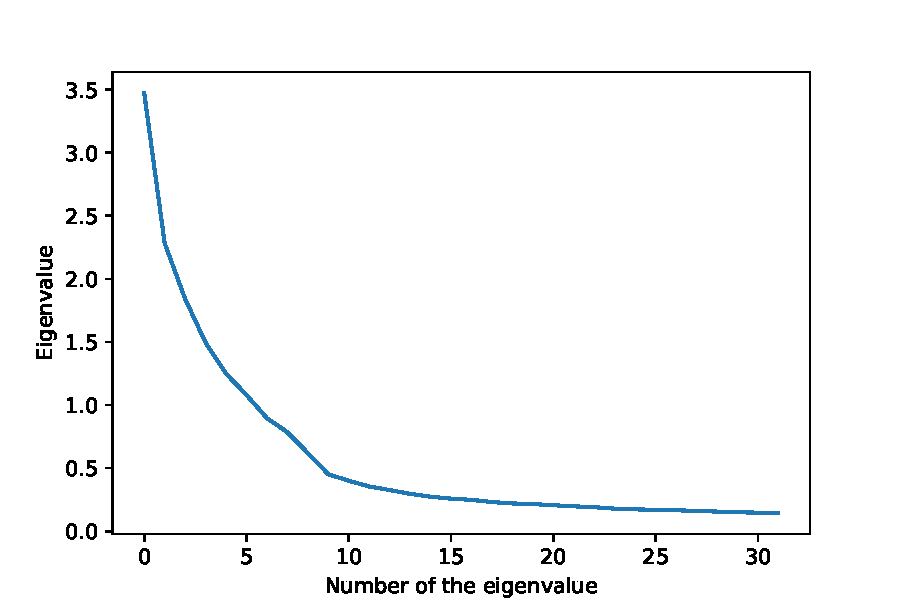
\includegraphics[width=0.74\textwidth]{img/eigenvalues.pdf}}
  \caption{Dependence of eigenvalues on their index in descending order.}
  \label{fig:evgen}
\end{figure}

Concretely, let
$$\mathbf{V} = \left\{ \mathbf{e}_1, \dots, \mathbf{e}_d \right\}, \qquad \bP = \left[ \mathbf{e}_1, \dots, \mathbf{e}_d \right],$$
be the corresponding eigenvectors (forming an eigenbasis) with the largest eigenvalues. Then, we represent the network parameters as
$$\bw = \bw^* + \bP\,\btheta,$$ where $\btheta \in \mathbb{R}^d$ denotes the coordinates in this reduced subspace. This representation
allows us to focus on the most significant directions, leading to a more tractable approximation of the loss landscape.

Substituting $\bw = \bw^* + \bP\,\btheta$ into the second-order Taylor approximation of the loss function, we obtain
$$\cL_k\bigl(\bw^* + \bP\,\btheta\bigr) \approx \cL_k\bigl(\bw^*\bigr) + \frac{1}{2}\,\btheta^{\T} \left( \bP^{\T}\,
  \bH_k\bigl(\bw^*\bigr)\,\bP \right) \btheta.$$
Define
$$\bLambda_k(\bw) := \bP^{\T}\,\bH_k(\bw)\,\bP, \quad \text{so that} \quad \bLambda_k(\bw^*) =
  \operatorname{diag}\bigl(\lambda_k^1,\dots,\lambda_k^d\bigr),$$
where $\lambda_k^1, \dots, \lambda_k^d$ are the top $d$ eigenvalues of $\bH_k(\bw^*)$. Thus, the loss is approximated as
$$\cL_k\bigl(\bw^* + \bP\,\btheta\bigr) \approx \cL_k\bigl(\bw^*\bigr) + \frac{1}{2}\,\btheta^{\T} \bLambda_k \btheta.$$

Similarly, for the loss computed on $k+1$ samples, we have
$$\cL_{k+1}\bigl(\bw^* + \bP\,\btheta\bigr) \approx \cL_{k+1}\bigl(\bw^*\bigr) + \frac{1}{2}\,\btheta^{\T} \bLambda_{k+1} \btheta.$$

\begin{theorem}
  (Of Delta-function) Let $p(\btheta)$ be a probability distribution over the reduced subspace (for instance, a Gaussian distribution), with mean
  $\bm = \mathbf{0}$ and covariance $\bSigma = \mathbb{D}_{p(\btheta)}\bigl(\btheta\bigr).$ Then,
  $$\Delta_k \;\approx\; \frac{\sigma^4}{4} \left( 2 \sum_{i=1}^{d}\left( \lambda_{k+1}^i - \lambda_{k}^i \right)^2 + \left(
      \sum_{i=1}^{d}\left( \lambda_{k+1}^i - \lambda_{k}^i \right) \right)^2 \right).$$
\end{theorem}

Assuming $\mathbb{E}_{p(\btheta)}(\btheta) = \mathbf{0}$ is natural when centering the sampling distribution at the minimum.

The result shown on this theorem and applied to our $p(\btheta)$ can estimate the $\Delta_k$ function so we can seay when the dataset
size will be sufficient.

\section{Experiments}
To verify the theoretical estimates, in this section, we present experiments aimed at analyzing how the loss landscape evolves as
the size of the training set increases.

\paragraph{Data.}
We use the MNIST \cite{deng2012mnist} and Fashion-MNIST \cite{xiao2017fashion} dataset, which consists of $60{,}000$
training images and $10{,}000$ test
images of handwritten digits (0--9). Each image is $28\times28$ pixels, grayscale.

\paragraph{Model Architecture.}
We use the following neural network model structures and fixations:
\begin{itemize}
  \item A multilayer perceptron (MLP) with different number of hidden layers (ReLU activations).
  \item The choice of architecture remains consistent across all experiments.
\end{itemize}


The first two are preliminary experiments, conducted as illustrative examples on the MNIST dataset,
while the others focusing on Hessian-based projections and show connections between eigenvalues and loss function convergence.
That is our primary aim --- to check our theoretical estimates in-deal. All experiments are avaliable at our github repository.

\subsection{Visualizing the Loss Landscape in a Random Two-Dimensional Subspace}
The idea of this initial experiment is to get an intuitive sense of how the loss function’s landscape shifts with
different training-set sizes. To do this, we pick two random directions $\mathbf{v}_1$ and $\mathbf{v}_2$ in the parameter
space and project the network’s parameters onto the subspace they span.

In order to visualize how the loss function behaves as the model parameters change along two chosen random directions, we compute loss
values over a two-dimensional grid in the projected parameter space. Recall that, in our setup, the loss function is defined as
$$L_k(w)=\frac{1}{k}\sum_{i=1}^{k}\ell_i(w),$$
where $\ell_i(w)$ is the loss contribution of the $i$th sample.

The procedure for computing the loss values and visualizing them in 3D is as follows:

\begin{enumerate}
  \item \textbf{Fix a base model and directions.}
        Begin with a fixed trained on the same dataset neural network model.
        Also, obtain two parameter directions $\btheta = \{\bv_1$, $\bv_2$\} that will be used to explore the parameter space.
        These directions are vectors in the model's parameter space.

  \item \textbf{Grid Construction.}
        We generate a two-dimensional grid of coefficient pairs $(\alpha,\beta)$ using a fixed step size within the interval $[-1,1]$.
        These coefficients will scale two pre-computed directions in the parameter space. The grid is formed by taking the Cartesian product.

  \item \textbf{Loss Calculation on the Grid.}
        For each grid point $(\alpha,\beta)$, a new set of parameters is created by forming a linear combination of the two directions:
        $$
          \btheta = \alpha\cdot\bv_1 + \beta\cdot\bv_2.
        $$
        A temporary model is then initialized with these shifted parameters, and combined with the base model via straight sum:
        $$\bw = \bw^* + \btheta$$.
        The base model's parameters are kept fixed (close to $\mathbf{w}^*$) while applying these perturbations.
        Using a loss function evaluation, the losses are computed for each grid point.

  \item \textbf{Computation of Aggregated Loss Measures.}
        The loss values for each grid point are aggregated in two ways:
        \begin{itemize}
          \item The mean loss $\cL_k$ computed over a specified number of samples is used to construct the loss landscape.
          \item Similarly, the mean loss $\cL_{k+1}$ for a larger sample size is computed, and the squared difference
                $$\left(\mathcal{L}_{\text{k+1}} - \mathcal{L}_{\text{k}}\right)^2$$
                is evaluated at each grid point.
        \end{itemize}

  \item \textbf{3D Surface Visualization.}
        Two 3D surface plots are created and placed side by side:
        \begin{itemize}
          \item \emph{Left Plot:} Displays the loss landscape $\mathcal{L}_{k}(\btheta)$, where the $x$ and $y$ axes correspond to the grid
                coordinates (the scaling coefficients along the two directions) and the $z$-axis shows the average loss value.
          \item \emph{Right Plot:} Shows the squared loss difference, $\left(\mathcal{L}_{k+1}(\btheta)-\mathcal{L}_{k}(\btheta)\right)^2$.
                This plot emphasizes regions where an additional data sample induces substantial changes in the loss.
        \end{itemize}
\end{enumerate}

\begin{figure}[!htbp]
  \hspace*{-2.2cm}
  \subfloat{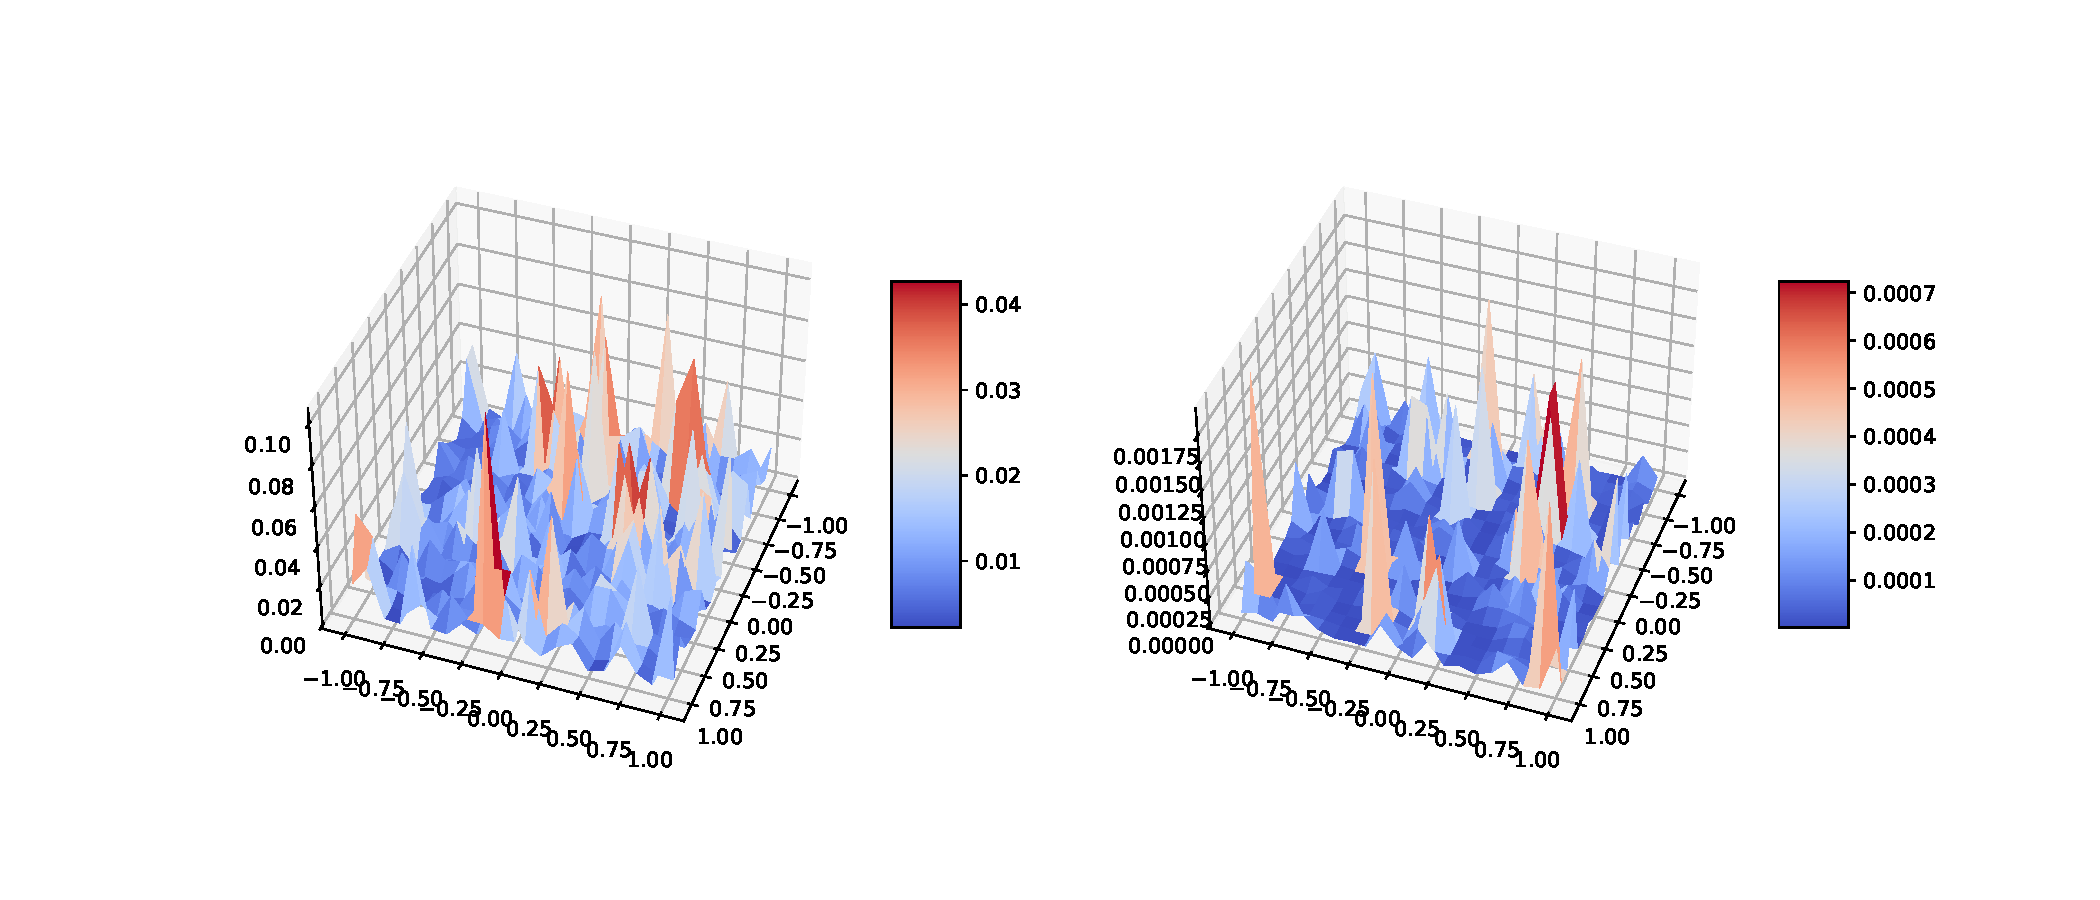
\includegraphics[width=1.3\textwidth]{img/loss_random_1_2.pdf}}
  \caption{Loss function landscape for small $k$}
  \label{fig:loss_random_small}
\end{figure}

\begin{figure}[!htbp]
  \hspace*{-2.2cm}
  \subfloat{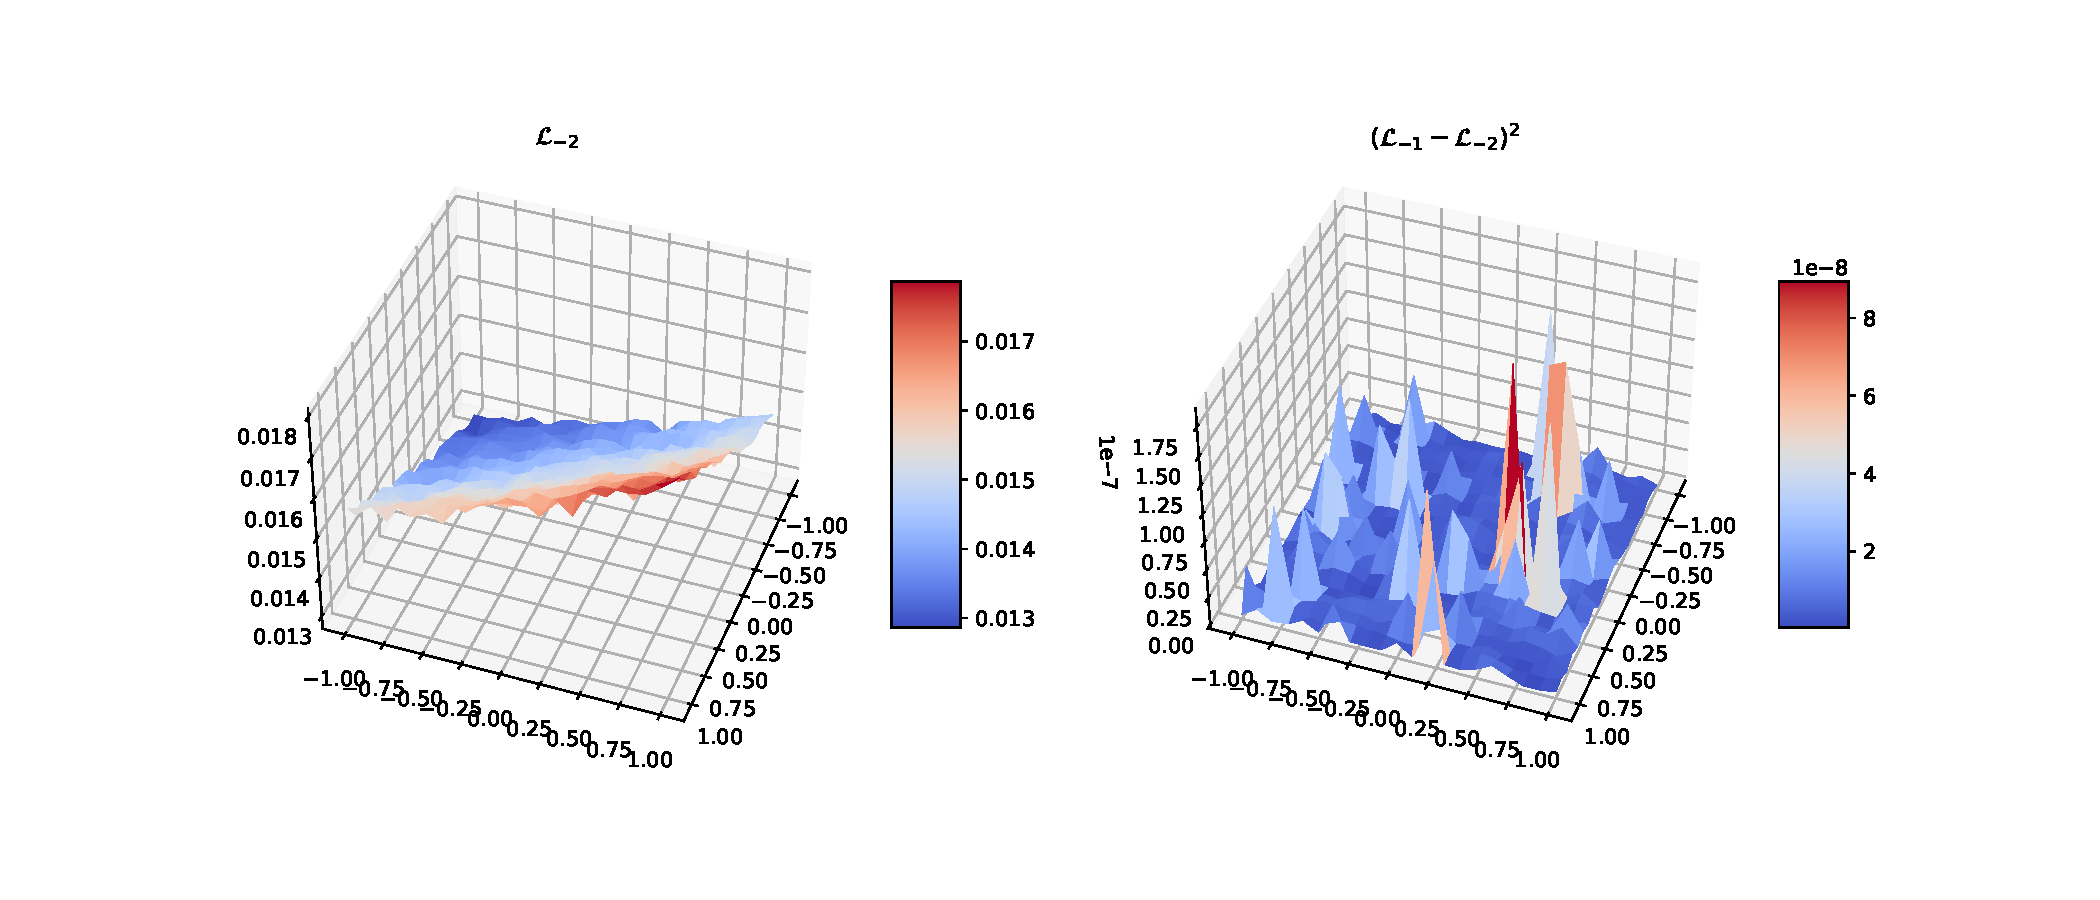
\includegraphics[width=1.3\textwidth]{img/loss_random_-2_-1.pdf}}
  \caption{Loss function landscape for maximum $k$}
  \label{fig:loss_random_big}
\end{figure}

Figures \ref{fig:loss_random_small} and \ref{fig:loss_random_big} shows a set of four 3D plots that illustrate the loss
landscape and the corresponding loss difference for various sample sizes. In these figures, the top two plots correspond to very small
training sets, while the bottom two plots display the loss landscape and its squared difference for the maximum available dataset size.

\paragraph{Loss Landscape for Small Sample Sizes}
In the upper plots \ref{fig:loss_random_small} ($k=1$), the loss landscape exhibits sharp variations and high-contrast peaks.
These characteristics indicate that when training with an extremely limited number of samples, the model is highly sensitive to small
perturbations in the parameter space. In such cases, even a slight change in parameters leads to significant fluctuations in the loss
function. This is further supported by the upper plot of the squared loss difference,
$$\left(\cL_k(\btheta)-\cL_{k}(\btheta)\right)^2,$$
which shows large local differences that reflect high instability in the optimization landscape.

\paragraph{Loss Landscape for Maximum Dataset Size}
In contrast, the lower plots \ref{fig:loss_random_big} correspond to training with the maximum available dataset size. Here, the loss
surface appears much smoother and more regular. The sharp peaks have diminished considerably, and the surface displays a gradual slope.
This smoothing of the loss landscape indicates that as more data become available, the model's local optimum stabilizes. Likewise, the
squared loss difference in the lower plot is much smaller, implying that the addition of extra samples produces only minor adjustments
to the loss function. Such convergence suggests that the network has captured the underlying data structure adequately, and that further
increases in the training sample size yield diminishing returns in terms of reshaping the loss landscape.

\subsection{Visualizing delta-function}

To further analyze the convergence of the loss landscape, we also evaluate and visualize the $\Delta_k$ function. This function 
quantifies the change in the loss function when transitioning from a model trained on $k$ samples to one trained on $k+1$ samples. 
Directly computing the expectation
$$\Delta_k = \mathbb{E}_{p(\bw)}\left( \cL_{k+1}(\bw) - \cL_{k}(\bw) \right)^2$$
over the entire distribution of parameter shifts is computationally infeasible. Therefore, we employ a Monte Carlo approximation, 
where we average the loss differences computed on a set of random Gaussian perturbations. This Monte Carlo approach is straightforward 
to implement and does not require explicit knowledge of the full distribution of parameter shifts.

The overall procedure is as follows:

\begin{enumerate}
  \item \textbf{Fixing a model and sampling Directions.}
        Begin with a fixed trained on the same dataset neural network model. Generate $K$ independent random directions from a
        multivariate normal distribution
        $$\btheta \sim \mathcal{N}(\bm, \sigma^2 \bI),$$
        where $\bm = \mathbf{0}$ and $\sigma$ as variance. These $K$ samples serve as the shifts in the reduced parameter space.

  \item \textbf{Parameter Snapshot.}\\
        For each random direction, form a perturbed parameter vector around the base parameter $\mathbf{w}^*$:
        $$\mathbf{w}^{(t)} = \mathbf{w}^* + \btheta^{(t)}, \quad t=1,\dots,K.$$
        The base model's parameters are kept fixed (close to $\mathbf{w}^*$) while applying these perturbations.

  \item \textbf{Loss Evaluation.}\\
        For each perturbed parameter $\mathbf{w}^{(t)}$, compute the loss values
        $$\cL_{k+1}(\mathbf{w}^{(t)}) \quad \text{and} \quad \cL_{k}(\mathbf{w}^{(t)}),$$
        and then calculate the squared loss difference
        $$\left( \cL_{k+1}(\mathbf{w}^{(t)}) - \cL_{k}(\mathbf{w}^{(t)}) \right)^2.$$

  \item \textbf{Averaging.}\\
        Average the squared loss differences over the $K$ samples to obtain the Monte Carlo estimate:
        $$\Delta_k \approx \frac{1}{K} \sum_{t=1}^{K} \left( \cL_{k+1}(\mathbf{w}^{(t)}) - \cL_{k}(\mathbf{w}^{(t)}) \right)^2.$$
        Increasing $K$ results in a more reliable estimate of the expected loss difference.

  \item \textbf{Visualization.}\\
        The computed $\Delta_k$ values are then visualized as follows:
        \begin{itemize}
          \item The left plot displays the evolution of $\Delta_k$ across different sample sizes. The $x$-axis represents the sample index $k$, while the $y$-axis shows the corresponding $\Delta_k$.
          \item The right plot shows the product $\Delta_k \cdot k^2$ (or another suitable scaling), which highlights the convergence rate of the loss differences as the dataset size increases.
        \end{itemize}
        These 2D plots are generated side-by-side to facilitate a comparative analysis of the convergence behavior.

\end{enumerate}

\begin{figure}[!htbp]
  \hspace*{-2.8cm}
  \subfloat{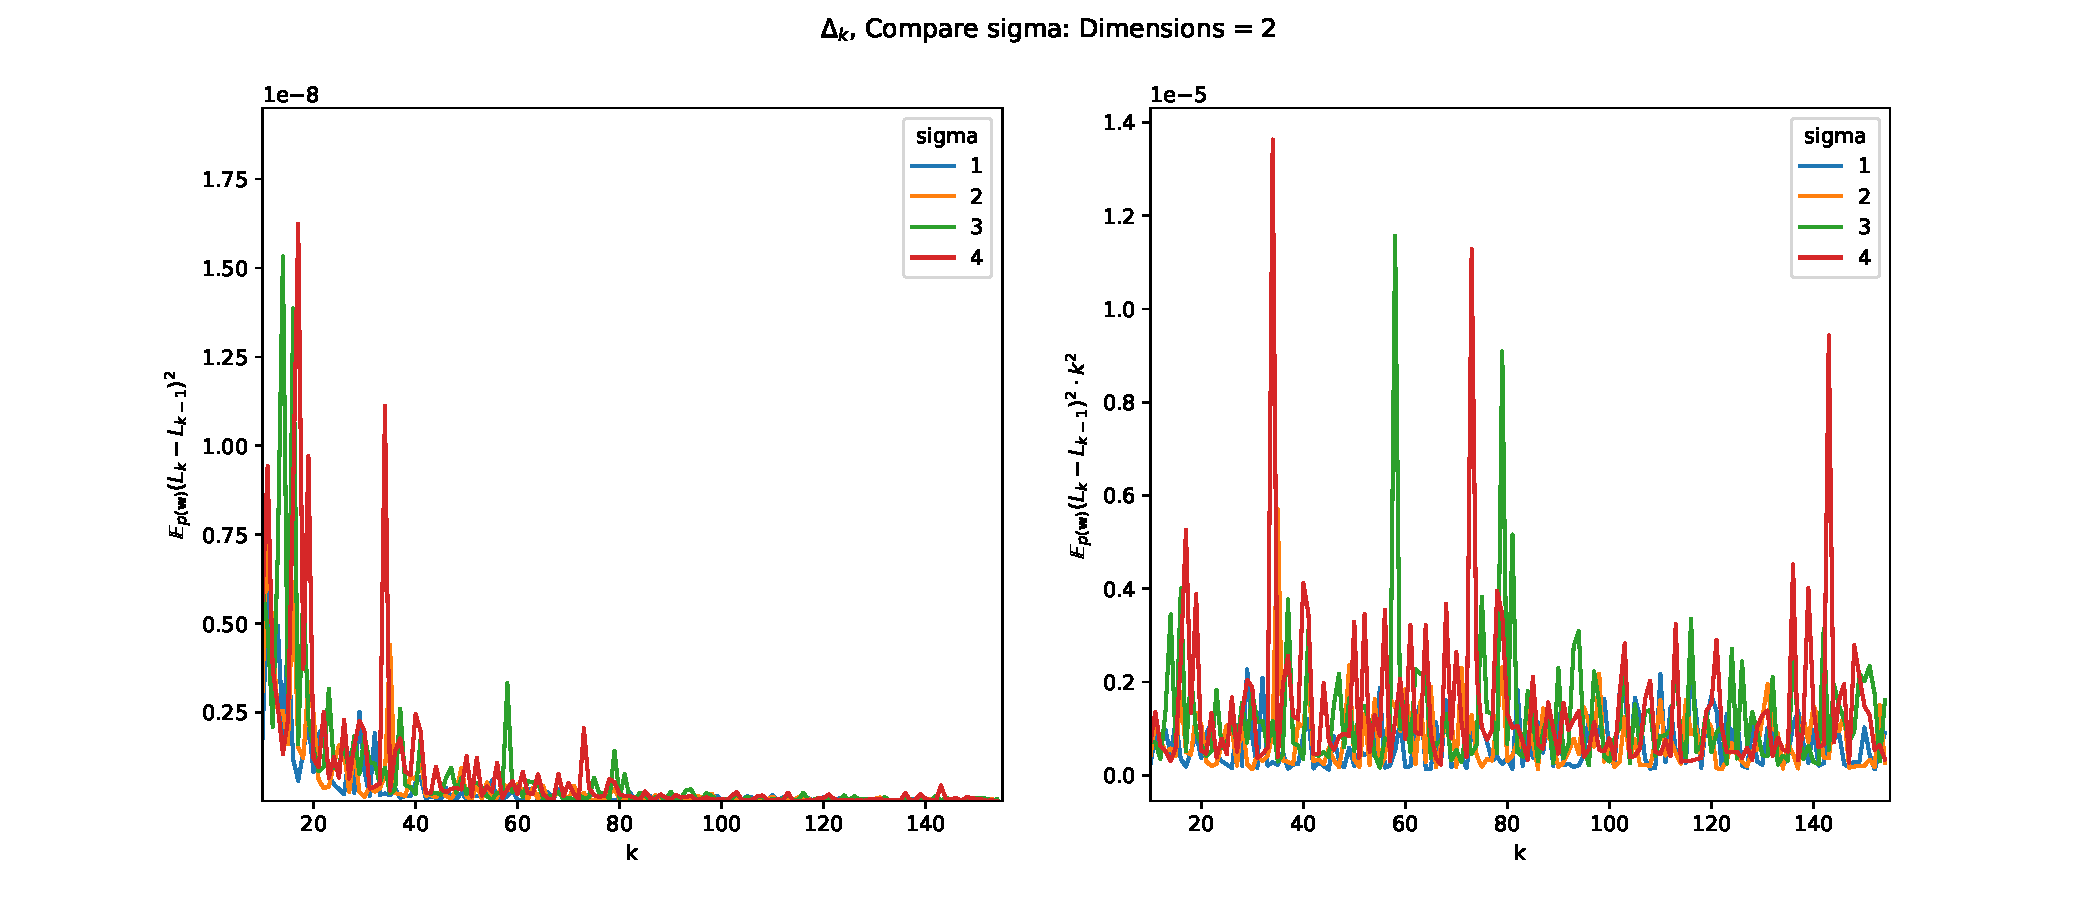
\includegraphics[width=1.35\textwidth]{img/delta_random_sigma_2_64.pdf}}
  \caption{Delta function landscape for different variation}
  \label{fig:delta_random_sigma}
\end{figure}

\begin{figure}[!htbp]
  \hspace*{-2.8cm}
  \subfloat{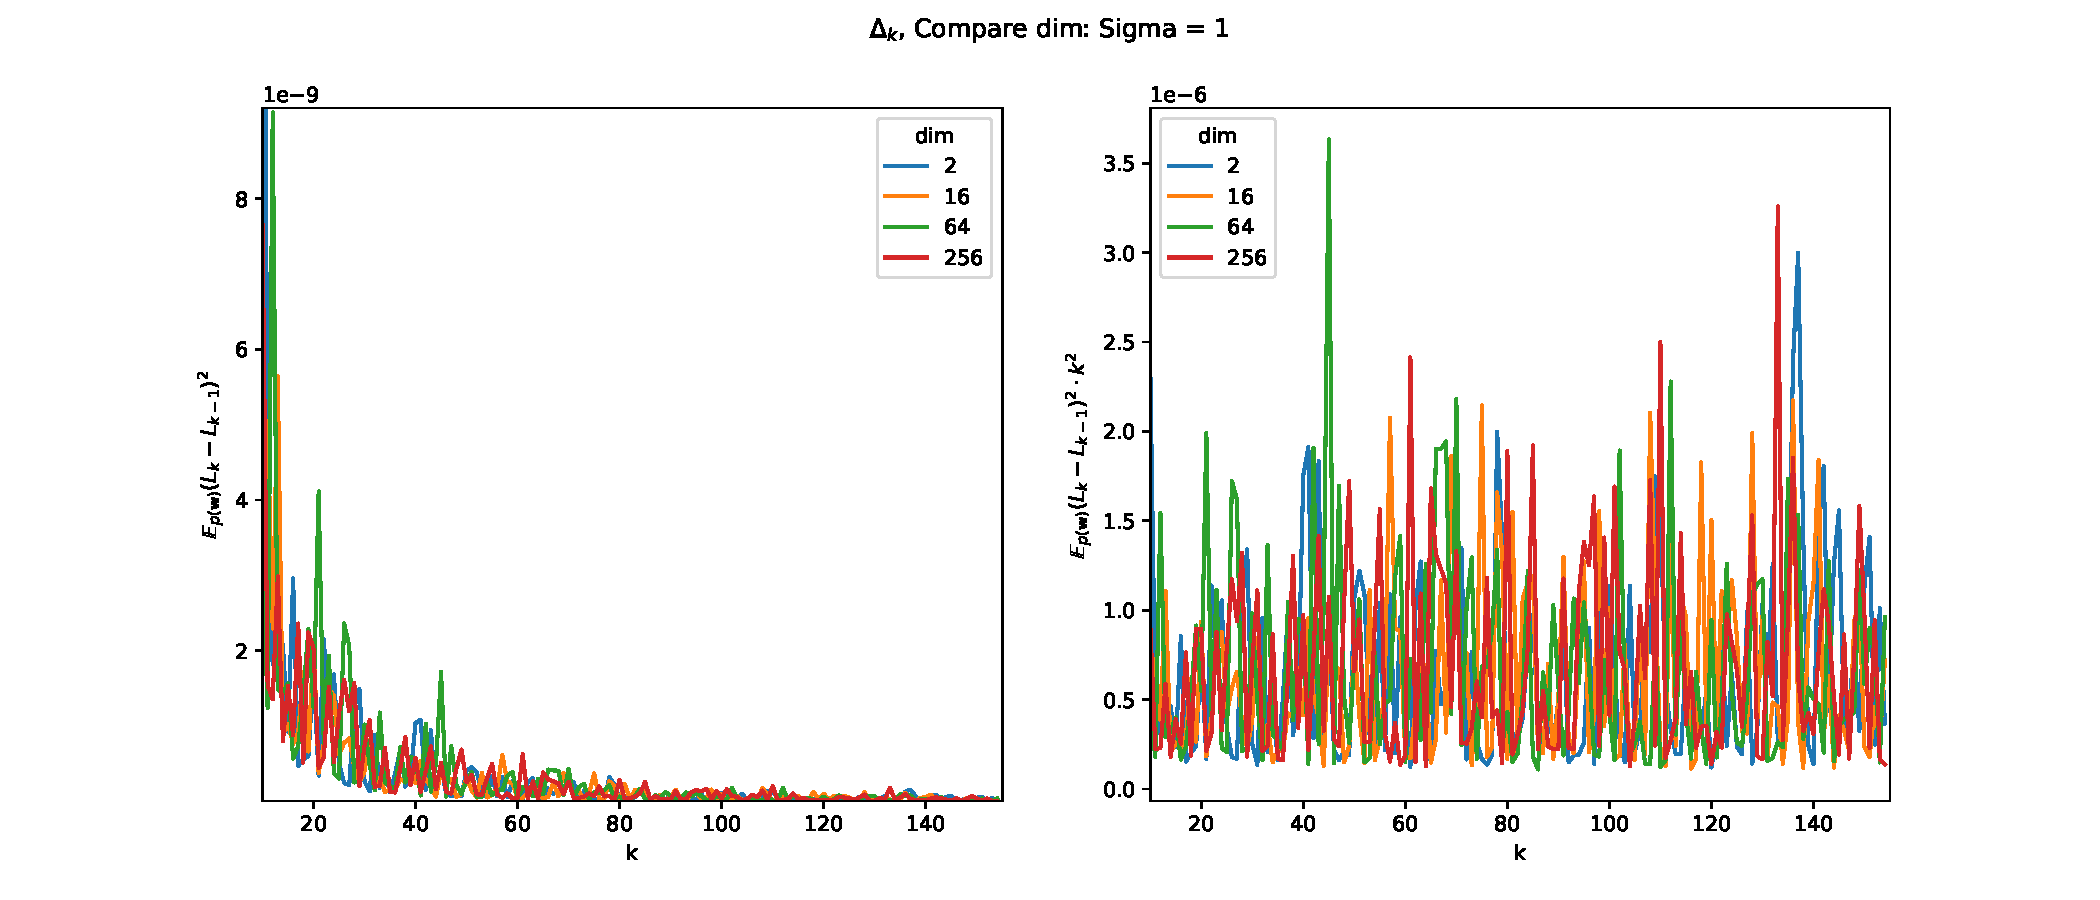
\includegraphics[width=1.35\textwidth]{img/delta_random_dim_1_64.pdf}}
  \caption{Delta function landscape for different number of dimensions}
  \label{fig:delta_random_dim}
\end{figure}

\begin{figure}[!htbp]
  \hspace*{-2.8cm}
  \subfloat{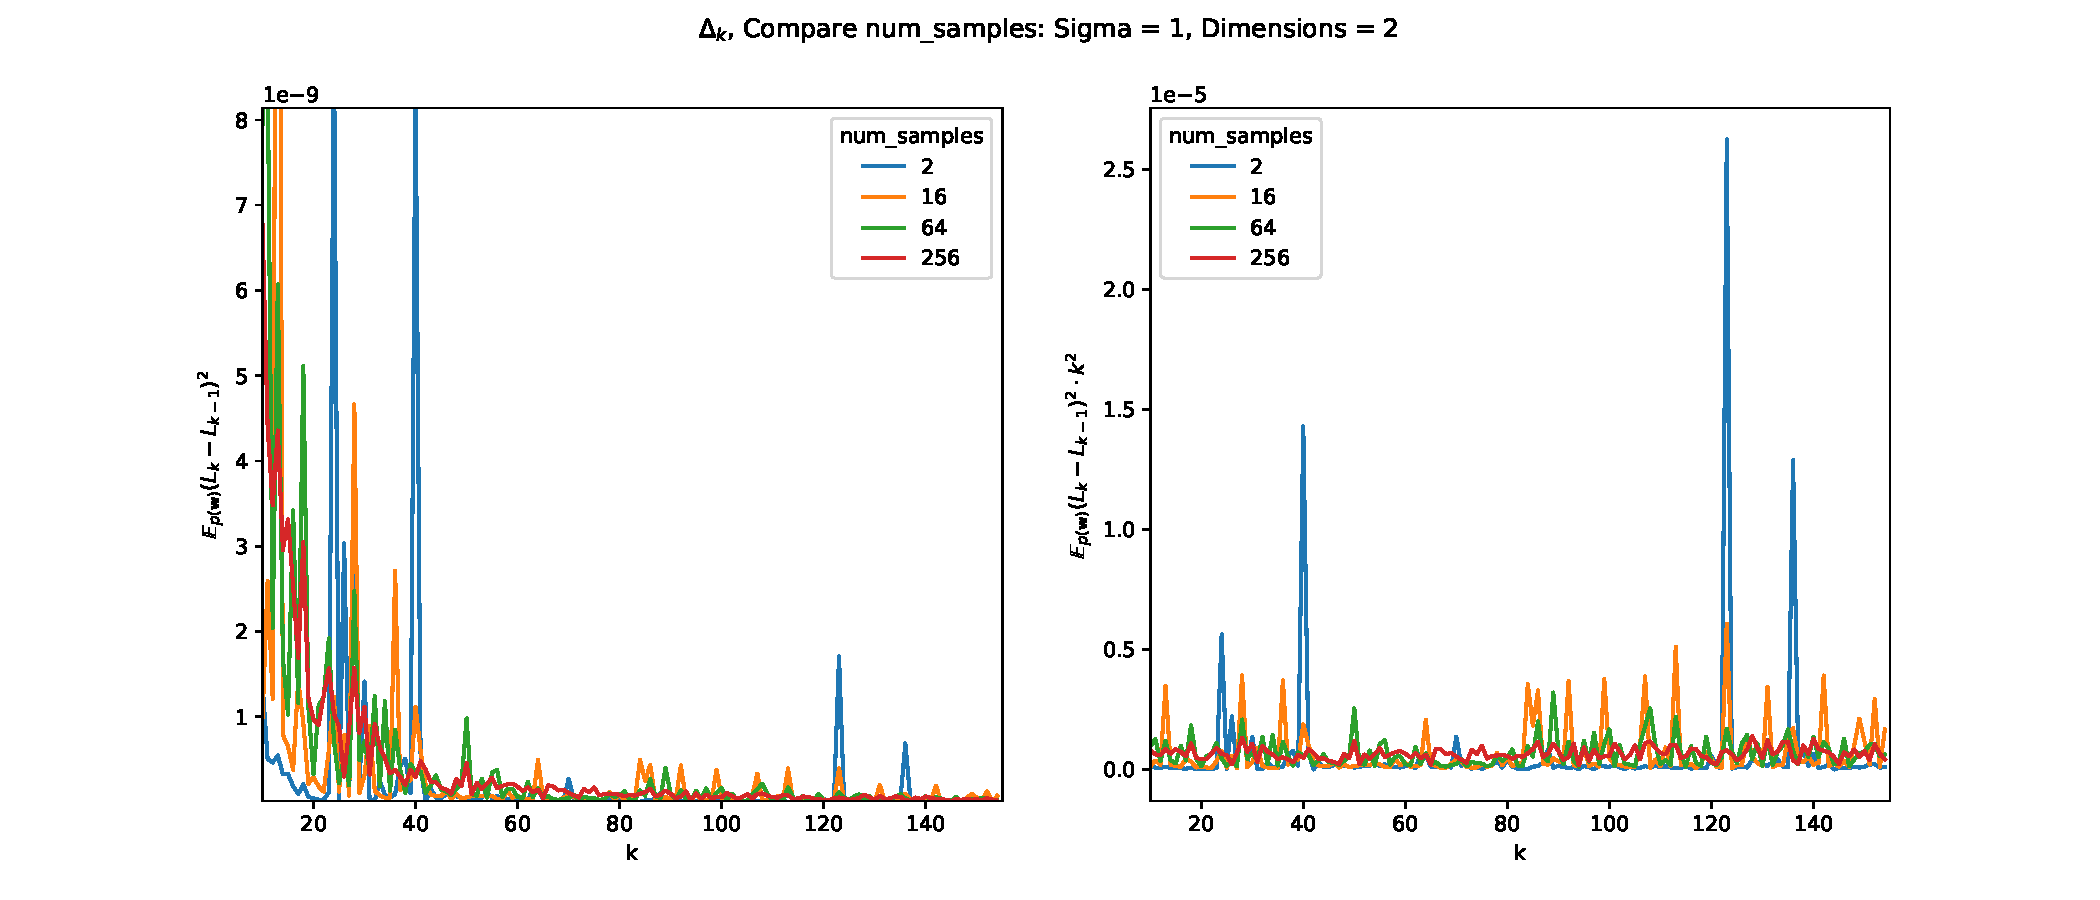
\includegraphics[width=1.35\textwidth]{img/delta_random_num_samples_1_2.pdf}}
  \caption{Delta function landscape for different number of samples ($K$)}
  \label{fig:delta_random_samples}
\end{figure}


Figures \ref{fig:delta_random_sigma}, \ref{fig:delta_random_dim}, and \ref{fig:delta_random_samples} present the behavior of the function
$$\Delta_k \;=\; \mathbb{E}_{p(\bw)}\bigl[L_{k+1}(\bw) - L_k(\bw)\bigr]^2$$
under varying parameters of the Monte Carlo sampling and the subspace dimension used for projection. Each figure focuses on a 
specific comparison: \ref{fig:delta_random_sigma} --- different values of the Gaussian variance $\sigma$, 
\ref{fig:delta_random_sigma} -- different sizes of the projected subspace (i.e., different dimensions), and 
\ref{fig:delta_random_sigma} different numbers of random samples~$K$ in the Monte Carlo algorithm.

\paragraph{Comparing Different Variances \texorpdfstring{$\sigma$}{sigma}}
Figure~\ref{fig:delta_random_sigma} shows how the $\Delta_k$ curves evolve when using various values of $\sigma$ for the random 
directions. A larger $\sigma$ increases the magnitude and frequency of spikes in the curves. Intuitively, when the Gaussian sampling 
is more spread out (i.e., we sample directions farther from the base parameter $\bw^*$), the resulting perturbations can induce more 
significant changes in the loss. Thus, $\Delta_k$ can become highly volatile. By contrast, a smaller $\sigma$ keeps the sampled points 
closer to the minimum, making the changes in loss more localized and stable. In practice, choosing too large a $\sigma$ can obscure the 
structure around $\bw^*$ with excessive noise, while a smaller $\sigma$ focuses on the region near the local minimum, highlighting 
more relevant variations in the loss landscape.

\paragraph{Comparing Different Subspace Dimensions}
Figure~\ref{fig:delta_random_dim} compares the $\Delta_k$ function for different projection dimensions. 
As the dimension of the subspace grows, the curves tend to exhibit fewer extreme spikes. This suggests that by considering more 
directions in the parameter space, the Monte Carlo estimation captures a broader view of potential perturbations. Consequently, 
individual outliers affect the overall measure less dramatically, leading to more stable curves. 
But a plenty of directions have negligible eigenvalues and thus minimal impact on the loss, so this does not necessarily 
mean we should always use a high-dimensional subspace. The idea of focusing on the dominant directions 
(with the largest eigenvalues) helps strike a balance between computational feasibility and capturing the most significant variations 
in the loss function.

\paragraph{Comparing Different Numbers of Random Samples \texorpdfstring{$K$}{K}}
Figure~\ref{fig:delta_random_samples} illustrates the effect of varying $K$, the number of random Gaussian samples used for Monte Carlo 
estimation. With a larger $K$, the curves become less noisy and more stable. This is because the average
$$\frac{1}{K} \sum_{t=1}^{K} \Bigl(\cL_{k+1}(\bw^{(t)}) - \cL_k(\bw^{(t)})\Bigr)^2$$
is taken over a greater number of directions, thereby reducing variance in the estimate. 

In addition, the right-side plots in these figures show the scaled quantity $\Delta_k \cdot k^2$, revealing an approximate $1/k$ decay 
for the unscaled $\Delta_k$. This suggests that the incremental change in the loss function diminishes on the order of $1/k$ as $k$ 
increases, confirming that once a sufficiently large dataset is reached, additional samples have only a minor impact on the local loss 
landscape.

\noindent
\textbf{Conclusion from Preliminary Experiments.}
These initial experiments demonstrate that the loss landscape becomes progressively more stable with increasing $N$.
However, the directions used here are either random. This motivates a more rigorous approach in the \emph{main experiment}
below, where we focus specifically on the most critical directions of curvature --- those corresponding to the top
eigenvalues of the Hessian.

\subsection{Main Experiment: Projection onto Dominant Hessian Eigenvectors}

From prior work \cite{sagun2018empirical}, we know that only a few Hessian eigenvectors (those associated with the largest
eigenvalues) tend to capture the most significant curvature directions. By projecting onto these principal directions,
we can more precisely measure how the landscape the loss surface changes as $k$ increases.

\paragraph{Procedure}
\begin{enumerate}
  \item \textbf{Hessian approximation.} For each trained model, approximate
        the Hessian $\mathbf{H}$ or its dominant eigenvalues/eigenvectors. Techniques ???
  \item \textbf{Eigen-decomposition.} Identify the top $d$ eigenvectors $\{\mathbf{e}_1, \dots, \mathbf{e}_d\}$ with the
        largest eigenvalues.
  \item \textbf{Calculation and analization.} For each model, calculate a $\Delta$ fuction via the same way as in the second
        experiment (using Monte-Carlo) and visualize via plots.
\end{enumerate}

\paragraph{Goal and Expected Outcome}
\begin{itemize}
  \item By focusing on the directions of largest curvature, we expect a clearer
        measure of how the landscape of the loss surface changes with additional data.
  \item This approach should yield a more accurate estimate of the point at which the
        landscape effectively stabilizes, thus helping to pinpoint a minimum viable dataset size.
  \item By applying experiments we check our calculations above on the reality.
\end{itemize}



\section{Discussion}\label{sec:disc}

TADAAA!

\section{Conclusion}\label{sec:concl}

TADAAA!


%%%%%%%%%%%%%%%%%%%%%%%%%%%%%%%%%%%%%%%%%%%%%%%%%%%%%%%%%%%%

\bibliographystyle{unsrtnat}
\bibliography{references}

%%%%%%%%%%%%%%%%%%%%%%%%%%%%%%%%%%%%%%%%%%%%%%%%%%%%%%%%%%%%

\newpage
\appendix
\section{Appendix}

\subsection{Proof of the Theorem 1}

\begin{proof}
  The difference between the two losses is given by
  $$\cL_{k+1}(\bw) - \cL_k(\bw) \approx \Bigl[\cL_{k+1}(\bw^*) - \cL_k(\bw^*)\Bigr] + \frac{1}{2}\,\btheta^{\T}
    \Bigl( \bLambda_{k+1} - \bLambda_k \Bigr) \btheta.$$

  Now, we apply a second assumption regarding the $\Delta_k$ function in the context of the projection. Let $p(\btheta)$ be a probability
  distribution over the reduced subspace (for instance, a Gaussian distribution), with mean
  $$\bm = \mathbb{E}_{p(\btheta)}\bigl(\btheta\bigr)$$ and covariance $$\bSigma = \mathbb{D}_{p(\btheta)}\bigl(\btheta\bigr).$$
  Then, following \cite{petersen2012matrix} (see page 35), one can show that
  $$\mathbb{E}_{p(\btheta)} \Bigl[ \cL_{k+1}(\bw) - \cL_k(\bw) \Bigr] \approx \Bigl[ \cL_{k+1}(\bw^*) - \cL_k(\bw^*)\Bigr] +
    \frac{1}{2} \Bigl( \mathrm{Tr}(\bA\,\bSigma) + \bm^{\T}\,\bA\,\bm \Bigr),$$ where $$\bA := \bLambda_{k+1}(\bw^*) - \bLambda_k(\bw^*).$$
  Note that $\mathrm{Tr}(\bLambda_k) = \sum_{i=1}^{d} \lambda_k^i$ and, consequently,
  $$\mathrm{Tr}(\bA) = \sum_{i=1}^{d} \lambda_{k+1}^i - \sum_{i=1}^{d} \lambda_k^i.$$

  Assume further that the distribution in the reduced space is given by
  $$\btheta \sim \mathcal{N}\bigl(\bm,\sigma^2 \bI\bigr),$$
  so that $\bSigma = \sigma^2 \bI$. Then, according to \cite{petersen2012matrix} (page 43), the variance of the loss difference is
  $$\mathbb{D}_{p(\btheta)}\Bigl[ \cL_{k+1}(\bw) - \cL_k(\bw) \Bigr] =\frac{1}{4} \left( 2 \sigma^4\,\mathrm{Tr}(\bA^2) +
    4 \sigma^2\,\bm^{\T}\,\bA^2\,\bm \right).$$

  Finally, the overall measure $\Delta_k$ is defined as
  $$\Delta_{k} \;=\; \mathbb{D}_{p(\btheta)}\Bigl[ \cL_{k+1}(\bw) - \cL_k(\bw) \Bigr] + \left( \mathbb{E}_{p(\btheta)}
    \Bigl[ \cL_{k+1}(\bw) - \cL_k(\bw) \Bigr] \right)^{2}\,.$$
  Substituting the above expressions, we have
  $$\Delta_k \;\approx\; \frac{1}{4}\left( 2 \sigma^4\,\mathrm{Tr}(\bA^2) + 4 \sigma^2\,\bm^{\T}\,\bA^2\,\bm \right) + \Bigl(\cL_{k+1}(\bw^*) -
    \cL_k(\bw^*)\Bigr)^2$$ $$\quad\quad +\; 2\Bigl(\cL_{k+1}(\bw^*) - \cL_k(\bw^*)\Bigr)\cdot \frac{1}{2}\Bigl( \mathrm{Tr}(\bA\,\bSigma) +
    \bm^{\T}\,\bA\,\bm \Bigr) +\; \frac{1}{4}\Bigl( \mathrm{Tr}(\bA\,\bSigma) + \bm^{\T}\,\bA\,\bm \Bigr)^{2}\,.$$

  Assuming that $\bw^*$ is a local minimizer and remembering that $\bm = \mathbf{0}$, the above expression simplifies to
  $$\Delta_k \;\approx\; \frac{1}{4}\left( 2 \sigma^4\,\mathrm{Tr}(\bA^2) \right) + \frac{1}{4}\Bigl( \mathrm{Tr}(\bA\,\bSigma) \Bigr)^2\,.$$
  Since $\bSigma = \sigma^2 \bI$, it follows that
  $$\mathrm{Tr}(\bA\,\bSigma) = \sigma^2\,\mathrm{Tr}(\bA),$$
  and therefore,
  $$\Delta_k \;\approx\; \frac{\sigma^4}{4} \left( 2\,\mathrm{Tr}(\bA^2) + \Bigl(\mathrm{Tr}(\bA)\Bigr)^2 \right).$$
  Recalling that $$\mathrm{Tr}(\bA) = \sum\limits_{i=1}^{d}\left( \lambda_{k+1}^i - \lambda_{k}^i \right)$$ and
  $$\mathrm{Tr}(\bA^2) = \sum_{i=1}^{d}\left( \lambda_{k+1}^i - \lambda_{k}^i \right)^2,$$
  we obtain
  $$\Delta_k \;\approx\; \frac{\sigma^4}{4} \left( 2 \sum_{i=1}^{d}\left( \lambda_{k+1}^i - \lambda_{k}^i \right)^2 + \left(
      \sum_{i=1}^{d}\left( \lambda_{k+1}^i - \lambda_{k}^i \right) \right)^2 \right).$$
\end{proof}

\end{document}
